\documentclass{ximera}
\usepackage{epsfig}

\graphicspath{
  {./}
  {figures/}
}

\usepackage{epstopdf}
%\usepackage{ulem}
\usepackage[normalem]{ulem}

\epstopdfsetup{outdir=./}

\usepackage{morewrites}
\makeatletter
\newcommand\subfile[1]{%
\renewcommand{\input}[1]{}%
\begingroup\skip@preamble\otherinput{#1}\endgroup\par\vspace{\topsep}
\let\input\otherinput}
\makeatother

\newcommand{\EXER}{}
\newcommand{\includeexercises}{\EXER\directlua{dofile(kpse.find_file("exercises","lua"))}}

\newenvironment{computerExercise}{\begin{exercise}}{\end{exercise}}

%\newcounter{ccounter}
%\setcounter{ccounter}{1}
%\newcommand{\Chapter}[1]{\setcounter{chapter}{\arabic{ccounter}}\chapter{#1}\addtocounter{ccounter}{1}}

%\newcommand{\section}[1]{\section{#1}\setcounter{thm}{0}\setcounter{equation}{0}}

%\renewcommand{\theequation}{\arabic{chapter}.\arabic{section}.\arabic{equation}}
%\renewcommand{\thefigure}{\arabic{chapter}.\arabic{figure}}
%\renewcommand{\thetable}{\arabic{chapter}.\arabic{table}}

%\newcommand{\Sec}[2]{\section{#1}\markright{\arabic{ccounter}.\arabic{section}.#2}\setcounter{equation}{0}\setcounter{thm}{0}\setcounter{figure}{0}}
  
\newcommand{\Sec}[2]{\section{#1}}

\setcounter{secnumdepth}{2}
%\setcounter{secnumdepth}{1} 

%\newcounter{THM}
%\renewcommand{\theTHM}{\arabic{chapter}.\arabic{section}}

\newcommand{\trademark}{{R\!\!\!\!\!\bigcirc}}
%\newtheorem{exercise}{}

\newcommand{\dfield}{{\sf SlopeField}}

\newcommand{\pplane}{{\sf PhasePlane}}

\newcommand{\PPLANE}{{\sf PHASEPLANE}}

% BADBAD: \newcommand{\Bbb}{\bf}. % Package amsfonts Warning: Obsolete command \Bbb; \mathbb should be used instead.

\newcommand{\R}{\mbox{$\mathbb{R}$}}
\let\C\relax
\newcommand{\C}{\mbox{$\mathbb{C}$}}
\newcommand{\Z}{\mbox{$\mathbb{Z}$}}
\newcommand{\N}{\mbox{$\mathbb{N}$}}
\newcommand{\D}{\mbox{{\bf D}}}

\newcommand{\WW}{\mathcal{W}}

\usepackage{amssymb}
%\newcommand{\qed}{\hfill\mbox{\raggedright$\square$} \vspace{1ex}}
%\newcommand{\proof}{\noindent {\bf Proof:} \hspace{0.1in}}

\newcommand{\setmin}{\;\mbox{--}\;}
\newcommand{\Matlab}{{M\small{AT\-LAB}} }
\newcommand{\Matlabp}{{M\small{AT\-LAB}}}
\newcommand{\computer}{\Matlab Instructions}
\renewcommand{\computer}{M\small{ATLAB} Instructions}
\newcommand{\half}{\mbox{$\frac{1}{2}$}}
\newcommand{\compose}{\raisebox{.15ex}{\mbox{{\scriptsize$\circ$}}}}
\newcommand{\AND}{\quad\mbox{and}\quad}
\newcommand{\vect}[2]{\left(\begin{array}{c} #1_1 \\ \vdots \\
 #1_{#2}\end{array}\right)}
\newcommand{\mattwo}[4]{\left(\begin{array}{rr} #1 & #2\\ #3
&#4\end{array}\right)}
\newcommand{\mattwoc}[4]{\left(\begin{array}{cc} #1 & #2\\ #3
&#4\end{array}\right)}
\newcommand{\vectwo}[2]{\left(\begin{array}{r} #1 \\ #2\end{array}\right)}
\newcommand{\vectwoc}[2]{\left(\begin{array}{c} #1 \\ #2\end{array}\right)}

\newcommand{\ignore}[1]{}


\newcommand{\inv}{^{-1}}
\newcommand{\CC}{{\cal C}}
\newcommand{\CCone}{\CC^1}
\newcommand{\Span}{{\rm span}}
\newcommand{\rank}{{\rm rank}}
\newcommand{\trace}{{\rm tr}}
\newcommand{\RE}{{\rm Re}}
\newcommand{\IM}{{\rm Im}}
\newcommand{\nulls}{{\rm null\;space}}

\newcommand{\dps}{\displaystyle}
\newcommand{\arraystart}{\renewcommand{\arraystretch}{1.8}}
\newcommand{\arrayfinish}{\renewcommand{\arraystretch}{1.2}}
\newcommand{\Start}[1]{\vspace{0.08in}\noindent {\bf Section~\ref{#1}}}
\newcommand{\exer}[1]{\noindent {\bf \ref{#1}}}
\newcommand{\ans}{\textbf{Answer:} }
\newcommand{\matthree}[9]{\left(\begin{array}{rrr} #1 & #2 & #3 \\ #4 & #5 & #6
\\ #7 & #8 & #9\end{array}\right)}
\newcommand{\cvectwo}[2]{\left(\begin{array}{c} #1 \\ #2\end{array}\right)}
\newcommand{\cmatthree}[9]{\left(\begin{array}{ccc} #1 & #2 & #3 \\ #4 & #5 &
#6 \\ #7 & #8 & #9\end{array}\right)}
\newcommand{\vecthree}[3]{\left(\begin{array}{r} #1 \\ #2 \\
#3\end{array}\right)}
\newcommand{\cvecthree}[3]{\left(\begin{array}{c} #1 \\ #2 \\
#3\end{array}\right)}
\newcommand{\cmattwo}[4]{\left(\begin{array}{cc} #1 & #2\\ #3
&#4\end{array}\right)}

\newcommand{\Matrix}[1]{\ensuremath{\left(\begin{array}{rrrrrrrrrrrrrrrrrr} #1 \end{array}\right)}}

\newcommand{\Matrixc}[1]{\ensuremath{\left(\begin{array}{cccccccccccc} #1 \end{array}\right)}}



\renewcommand{\labelenumi}{\theenumi}
\newenvironment{enumeratea}%
{\begingroup
 \renewcommand{\theenumi}{\alph{enumi}}
 \renewcommand{\labelenumi}{(\theenumi)}
 \begin{enumerate}}
 {\end{enumerate}
 \endgroup}

\newcounter{help}
\renewcommand{\thehelp}{\thesection.\arabic{equation}}

%\newenvironment{equation*}%
%{\renewcommand\endequation{\eqno (\theequation)* $$}%
%   \begin{equation}}%
%   {\end{equation}\renewcommand\endequation{\eqno \@eqnnum
%$$\global\@ignoretrue}}

%\input{psfig.tex}

\author{Martin Golubitsky and Michael Dellnitz}

%\newenvironment{matlabEquation}%
%{\renewcommand\endequation{\eqno (\theequation*) $$}%
%   \begin{equation}}%
%   {\end{equation}\renewcommand\endequation{\eqno \@eqnnum
% $$\global\@ignoretrue}}

\newcommand{\soln}{\textbf{Solution:} }
\newcommand{\exercap}[1]{\centerline{Figure~\ref{#1}}}
\newcommand{\exercaptwo}[1]{\centerline{Figure~\ref{#1}a\hspace{2.1in}
Figure~\ref{#1}b}}
\newcommand{\exercapthree}[1]{\centerline{Figure~\ref{#1}a\hspace{1.2in}
Figure~\ref{#1}b\hspace{1.2in}Figure~\ref{#1}c}}
\newcommand{\para}{\hspace{0.4in}}

\usepackage{ifluatex}
\ifluatex
\ifcsname displaysolutions\endcsname%
\else
\renewenvironment{solution}{\suppress}{\endsuppress}
\fi
\else
\renewenvironment{solution}{}{}
\fi

\ifcsname answer\endcsname
\renewcommand{\answer}{}
\fi

%\ifxake
%\newenvironment{matlabEquation}{\begin{equation}}{\end{equation}}
%\else
\newenvironment{matlabEquation}%
{\let\oldtheequation\theequation\renewcommand{\theequation}{\oldtheequation*}\begin{equation}}%
  {\end{equation}\let\theequation\oldtheequation}
%\fi

\makeatother

\newcommand{\RED}[1]{{\color{red}{#1}}} 

\begin{document}

\noindent In Exercises~\ref{c9.4.3a} -- \ref{c9.4.3c}, 
consider the system of differential equations \eqref{E:duff}
\begin{matlabEquation}  \label{E:duff}
\begin{array}{rcl}
\dot{x} & = & y - \mu x - x^2   \\
\dot{y} & = & -x - \mu y + x^2.
\end{array}
\end{matlabEquation}
\begin{computerExercise} \label{c9.4.3a}
Show that \eqref{E:duff} undergoes a Hopf bifurcation near the origin when 
$\mu=0$.  Sketch the qualitative phase portraits on either 
side of the Hopf bifurcation.

\begin{solution}

The Jacobian of \eqref{E:duff} at the origin is
\[
J_{(0,0,\mu)} = \cmattwo{-\mu}{1}{-1}{-\mu}.
\]
Let $\mu = 0$.  Then $\trace(J_{(0,0,0)}) = -2\mu = 0$ and
$\det(J_{(0,0,0)}) = \mu^2 + 1 = 1 > 0$.  The trace moves through $0$ with
nonzero speed since
\[
\frac{d}{d\mu}\trace(J_{(0,0,0)}) = \frac{d}{d\mu}(-2\mu) = -2 \neq 0.
\]
Thus, \eqref{E:duff} undergoes a Hopf bifurcation near the origin when
$\mu = 0$.  Figure~\ref{c9.4.3a} shows the system with $\mu = 0.05$.  At
this point, the origin is a source.  Figure~\ref{c9.4.3b} shows the
system with $\mu = -0.05$.  At this point, the origin is a sink, and there
is a periodic solution.

\end{solution}
\end{computerExercise}
\begin{computerExercise} \label{c9.4.3b}
Show that another bifurcation takes place in \eqref{E:duff} near 
$\mu\approx -0.1$.  Sketch the new phase portrait that appears near this 
bifurcation.    

\begin{solution}

There is a homoclinic bifurcation at $\mu \approx -0.1$.  To show this,
compare Figure~\ref{c9.4.3b} with Figure~\ref{c9.4.3c}, which shows the
system with $\mu = -0.15$.  At $\mu = -0.15$, there is no longer a periodic
solution around the origin.  The bifurcation point occurs when the stable
and unstable orbits of the saddle point in the first quadrant coincide.

\end{solution}
\end{computerExercise}
\begin{computerExercise} \label{c9.4.3c}
For each of the three different phase portraits examined in 
Exercises~\ref{c9.4.3a} and \ref{c9.4.3b} identify the region of initial 
conditions in the square $-4\leq x,y \leq 4$ where solutions stay within the 
square in forward time and the region where solutions stay within the square 
in both forward and backward time.

\begin{solution}

When $\mu > 0$, all solutions with initial conditions between the
stable orbits of the saddle point stay within the square $-2 \leq
x,y \leq 2$ in forward time, and no solutions stay within this region
for all time.

\para When $-0.1 < \mu < 0$, all solutions with initial
conditions between the stable orbits of the saddle point stay within the
region in forward time.  Solutions with initial conditions inside the
periodic orbit stay within the region in backward time also.

\para When $\mu < -0.1$, only solutions with initial conditions along the
stable orbits of the saddle point stay within the region in forward time,
and no solutions stay within the region for all time.

\begin{figure}[htb]
                       \centerline{%
                       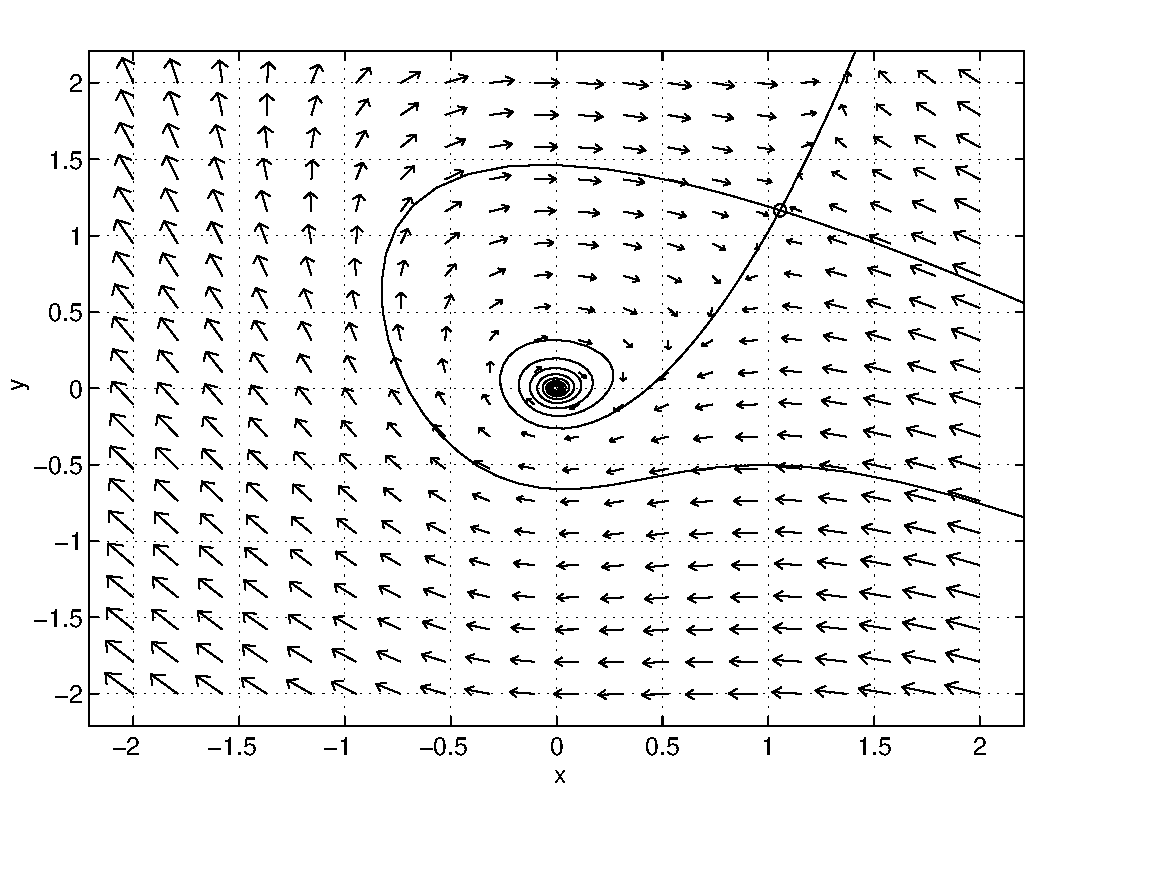
\includegraphics[width=1.8in]{exfigure/9-4-3a.pdf}
                       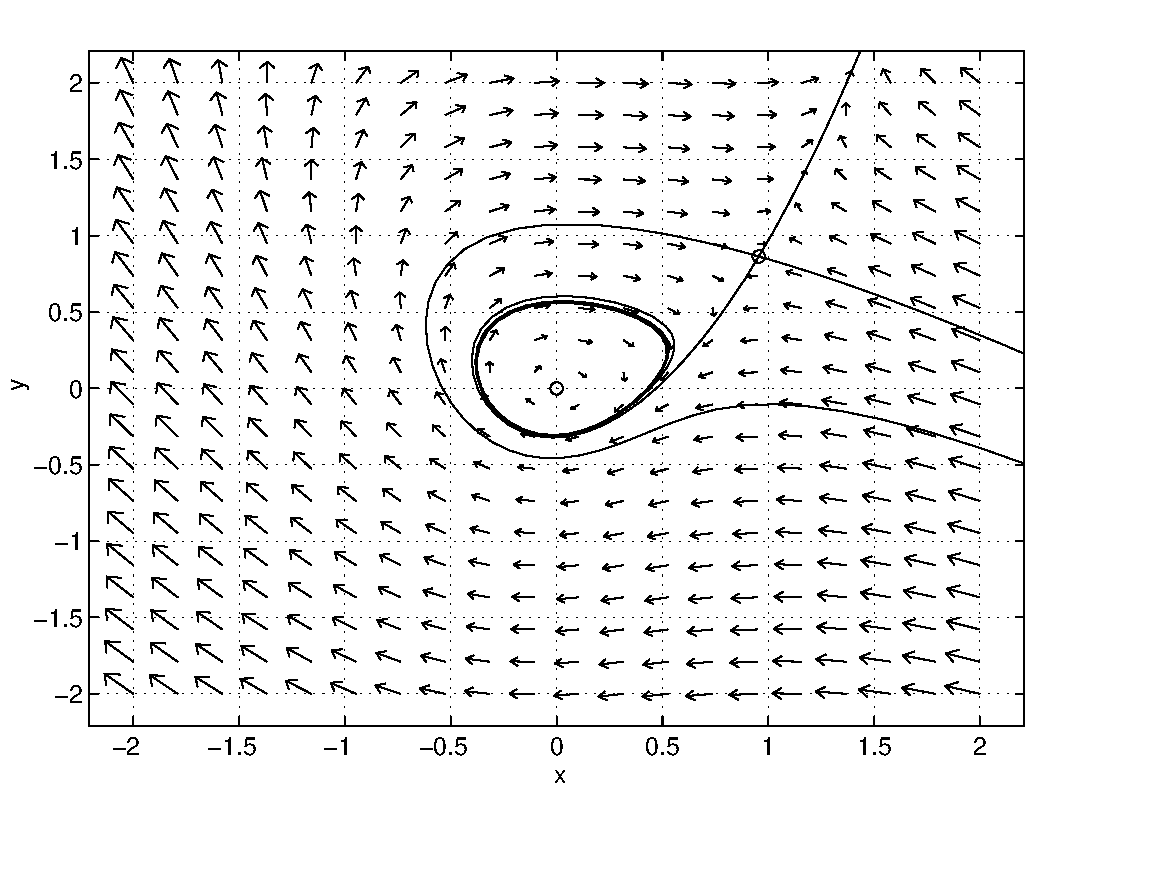
\includegraphics[width=1.8in]{exfigure/9-4-3b.pdf}
                       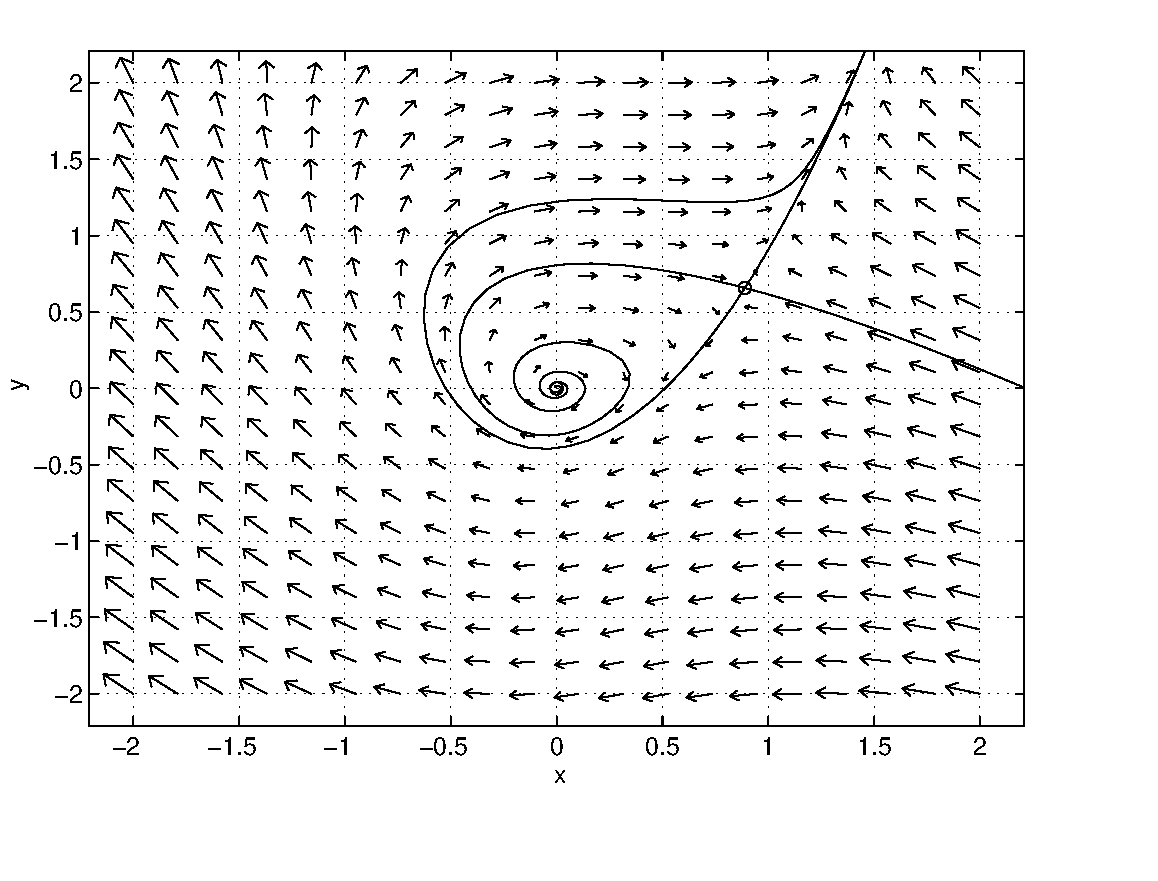
\includegraphics[width=1.8in]{exfigure/9-4-3c.pdf}}
		\centerline{$\mu > 0$\hspace{1.2in}$-0.1 < \mu < 0$
\hspace{1.2in}$\mu < -0.1$}
		\centerline{Figure~\ref{c9.4.3a}\hspace{1.2in}
Figure~\ref{c9.4.3b}\hspace{1.2in}Figure~\ref{c9.4.3c}}
\end{figure}

\end{solution}
\end{computerExercise}
\end{document}
